%=====================================================================
%  04-PENDAHULUAN.TEX
%=====================================================================
\section{PENDAHULUAN}

%---------------------------------------------------------------------
%  Slide contoh: qubit, representasi vektor, dan bola Bloch.
%  Perhatikan pola dua kolom: teks konsep di kiri, persamaan di kanan.
%---------------------------------------------------------------------
\begin{frame}
    \frametitle{Basic Quantum Information}
    \begin{columns}[T]
        \begin{column}{0.5\textwidth}
            \begin{itemize}\tiny
                \item Quantum Bit \\
                    \justifying
                    Dalam teori kuantum terdapat unit dasar informasi yang
                    disebut qubit: sistem kuantum dengan dua keadaan fisik
                    berbeda, direpresentasikan sebagai $\ket{0}$ dan
                    $\ket{1}$ \cite{barnett2009quantum}. Sifat superposisi
                    memungkinkan qubit berada pada perpaduan keduanya
                    secara bersamaan, melalui vektor dua dimensi
                    \begin{equation}
                        \ket{0}=\begin{bmatrix}1\\0\end{bmatrix},
                        \qquad
                        \ket{1}=\begin{bmatrix}0\\1\end{bmatrix}.
                        \label{eq:ket0-ket1}
                    \end{equation}                \item Bloch Sphere \\
                    \begin{minipage}[c]{0.30\textwidth}
                        \begin{figure}
                            \centering
                            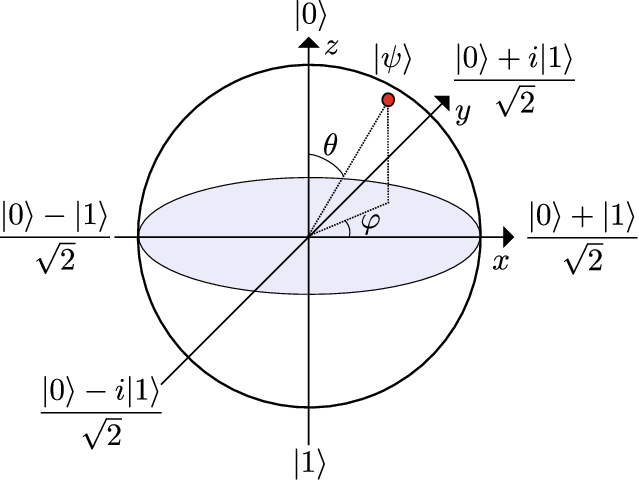
\includegraphics[width=0.62\textwidth]{gambar/BASIC/Bloch-Shapire.png}
                            \captionsetup{font=tiny}
                            \caption{Bola Bloch.}
                            \label{fig:bola-bloch}
                        \end{figure}
                    \end{minipage}%
                    \begin{minipage}[c]{0.66\textwidth}
                        \tiny\justifying Bola Bloch adalah representasi geometris
                        keadaan satu qubit; setiap titik pada permukaannya
                        mewakili satu keadaan kuantum murni yang mungkin,
                        dituliskan melalui
                        \begin{equation*}
                            \ket{\psi}=\cos(\theta/2)\ket{0}
                            +e^{i\phi}\sin(\theta/2)\ket{1}.
                        \end{equation*}
                    \end{minipage}
            \end{itemize}
        \end{column}

        \begin{column}{0.5\textwidth}\tiny
            \begin{equation*}
                \ket{\psi}
                    = \alpha\ket{0}+\beta\ket{1}
                    = \begin{bmatrix}\alpha\\ \beta\end{bmatrix}
            \end{equation*}

            \justifying
            dengan $|\alpha|^2+|\beta|^2=1$; $\ket{\psi}$ adalah titik pada
            permukaan \textit{bola Bloch} (Gambar~\ref{fig:bola-bloch}),
            $\theta$ sudut polar, $\phi$ sudut azimut.
        \end{column}
    \end{columns}
\end{frame}

\begin{frame}
    \frametitle{Quantum Entanglement}
    % Gambar ilustrasiFull-slide; caption menjelaskan konteksnya.
    \begin{figure}
        \centering
        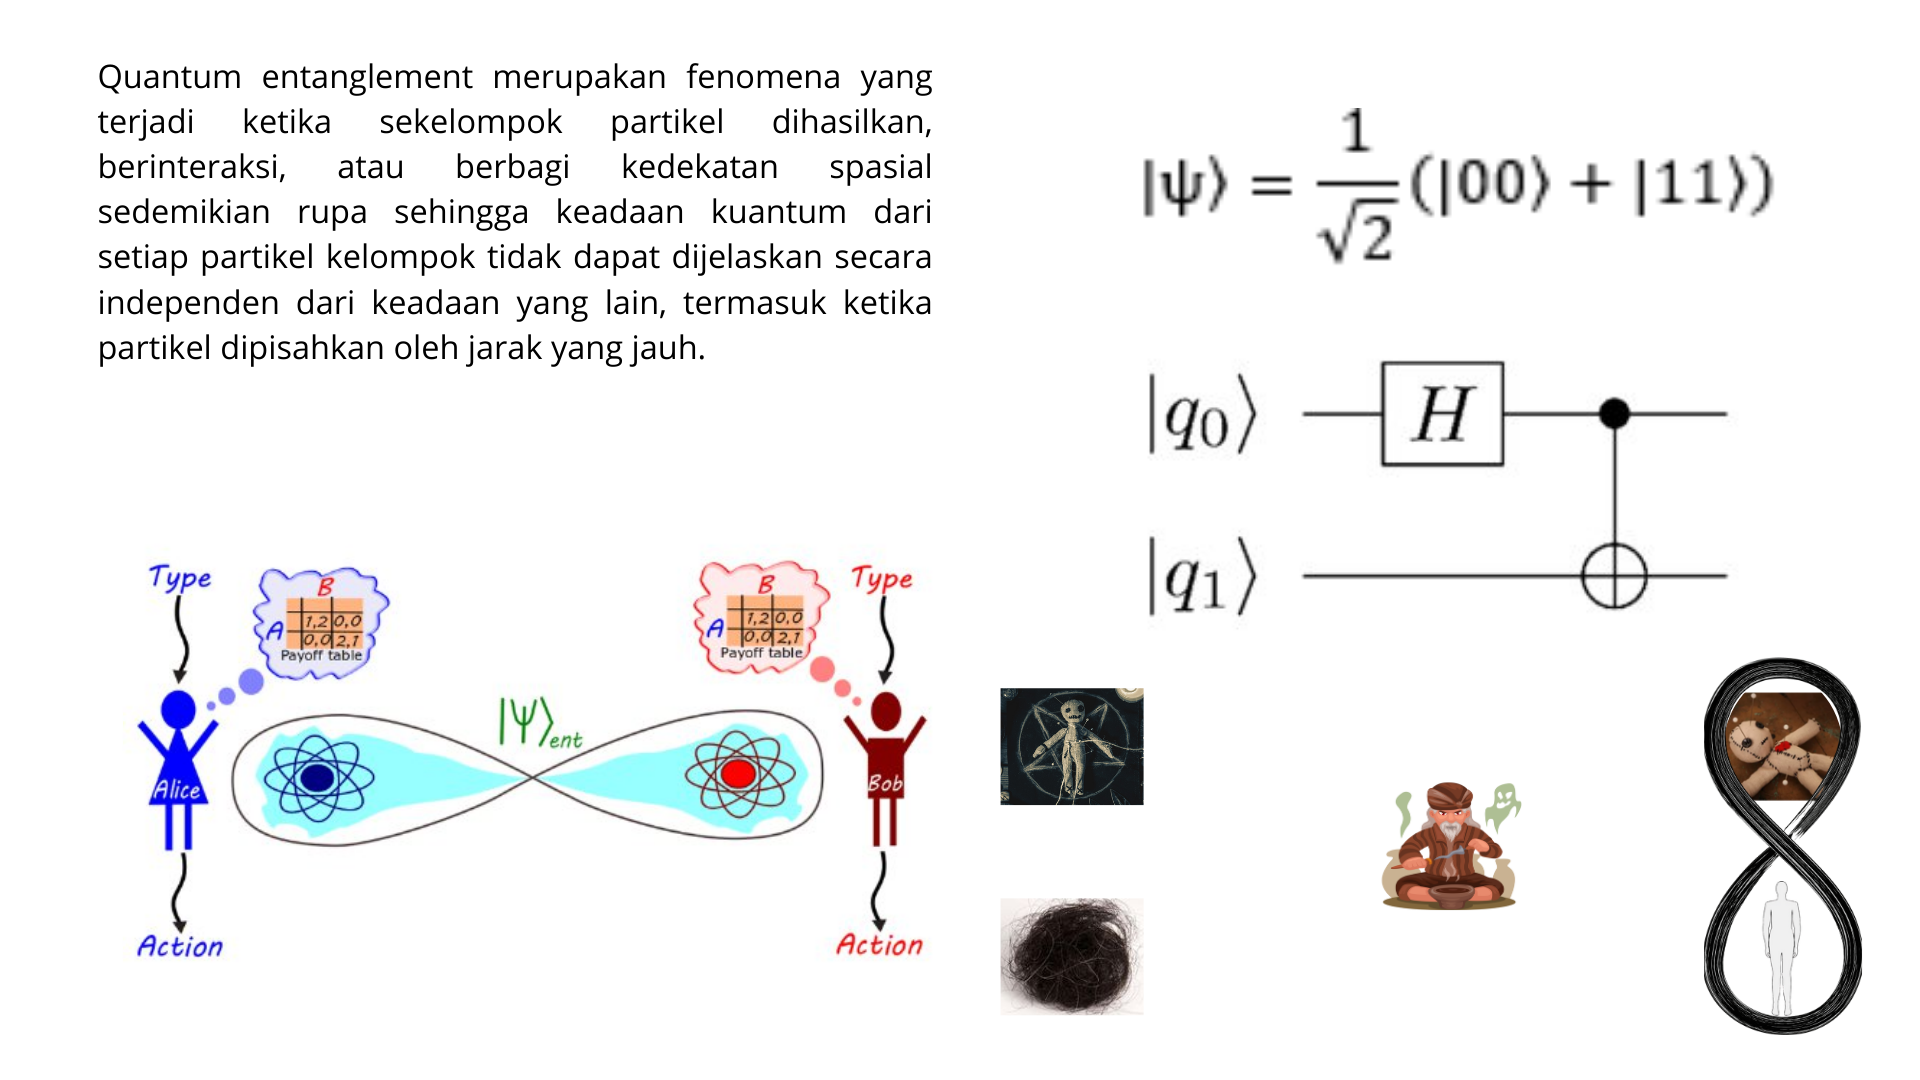
\includegraphics[width=0.66\textwidth]{gambar/BASIC/entanglement.png}
        \captionsetup{font=tiny, justification=justified}
        \captionof{figure}{Ilustrasi \textit{quantum entanglement}: sepasang
        partikel terjerat saling berkorelasi terlepas dari jarak pemisahnya.}
        \label{fig:entanglement-illustration}
    \end{figure}
\end{frame}
